\documentclass{standalone}
\usepackage{tikz}
\usetikzlibrary{patterns, positioning}


\begin{document}
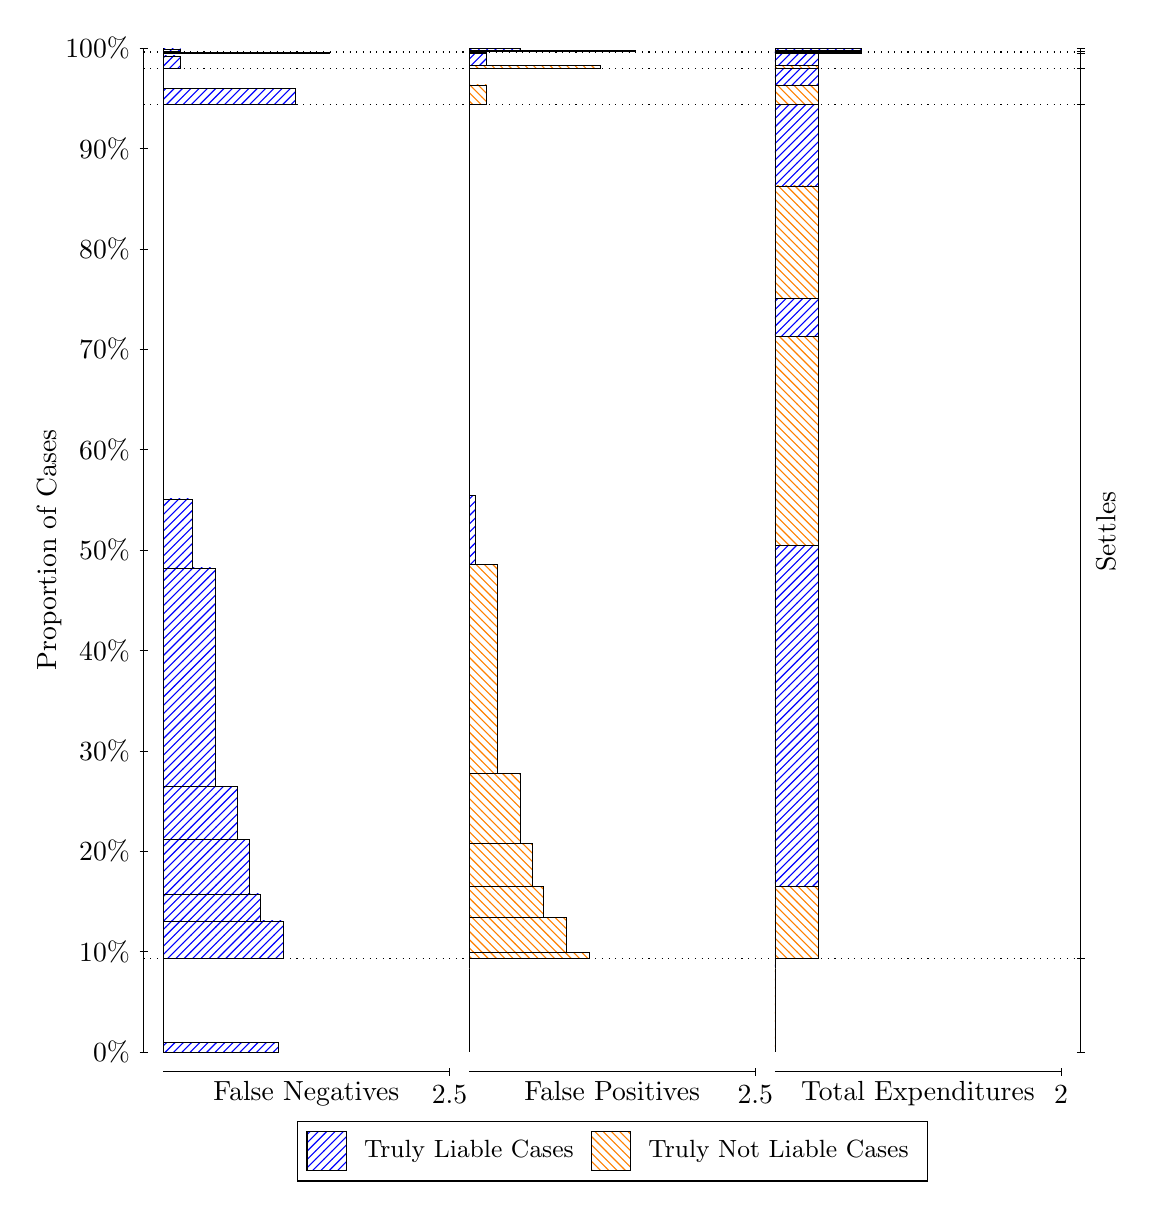
\begin{tikzpicture}
\draw[black, very thin] (1.5,1.75) -- (1.5,14.5);
\node[rotate=90, text=black, anchor=center] at (0.3, 8.125) {Proportion of Cases};
\draw[black, very thin] (1.45,1.75) -- (1.55,1.75);
\node[text=black, anchor=east] at (1.45, 1.75) {0\%};
\draw[black, very thin] (1.45,3.025) -- (1.55,3.025);
\node[text=black, anchor=east] at (1.45, 3.025) {10\%};
\draw[black, very thin] (1.45,4.3) -- (1.55,4.3);
\node[text=black, anchor=east] at (1.45, 4.3) {20\%};
\draw[black, very thin] (1.45,5.575) -- (1.55,5.575);
\node[text=black, anchor=east] at (1.45, 5.575) {30\%};
\draw[black, very thin] (1.45,6.85) -- (1.55,6.85);
\node[text=black, anchor=east] at (1.45, 6.85) {40\%};
\draw[black, very thin] (1.45,8.125) -- (1.55,8.125);
\node[text=black, anchor=east] at (1.45, 8.125) {50\%};
\draw[black, very thin] (1.45,9.4) -- (1.55,9.4);
\node[text=black, anchor=east] at (1.45, 9.4) {60\%};
\draw[black, very thin] (1.45,10.675) -- (1.55,10.675);
\node[text=black, anchor=east] at (1.45, 10.675) {70\%};
\draw[black, very thin] (1.45,11.95) -- (1.55,11.95);
\node[text=black, anchor=east] at (1.45, 11.95) {80\%};
\draw[black, very thin] (1.45,13.225) -- (1.55,13.225);
\node[text=black, anchor=east] at (1.45, 13.225) {90\%};
\draw[black, very thin] (1.45,14.5) -- (1.55,14.5);
\node[text=black, anchor=east] at (1.45, 14.5) {100\%};

\draw[black, very thin] (13.4,1.75) -- (13.4,14.5);
\draw[black, very thin] (13.35,1.75) -- (13.45,1.75);
\node[anchor=west] at (13.35, 1.75) {};
\draw[black, very thin] (13.35,2.9362) -- (13.45,2.9362);
\node[anchor=west] at (13.35, 2.9362) {};
\draw[black, very thin] (13.35,13.78) -- (13.45,13.78);
\node[anchor=west] at (13.35, 13.78) {};
\draw[black, very thin] (13.35,14.24) -- (13.45,14.24);
\node[anchor=west] at (13.35, 14.24) {};
\draw[black, very thin] (13.35,14.439) -- (13.45,14.439);
\node[anchor=west] at (13.35, 14.439) {};
\draw[black, very thin] (13.35,14.459) -- (13.45,14.459);
\node[anchor=west] at (13.35, 14.459) {};
\draw[black, very thin] (13.35,14.5) -- (13.45,14.5);
\node[anchor=west] at (13.35, 14.5) {};

\draw[black, very thin, pattern color=blue, pattern=north east lines] (1.75,1.75) rectangle (3.2033,1.8748);
\draw[black, very thin, pattern color=orange, pattern=north west lines] (1.75,1.8748) rectangle (1.75,2.9362);
\draw[black, very thin, pattern color=blue, pattern=north east lines] (1.75,2.9362) rectangle (3.276,3.4147);
\draw[black, very thin, pattern color=blue, pattern=north east lines] (1.75,3.4147) rectangle (2.9853,3.7582);
\draw[black, very thin, pattern color=blue, pattern=north east lines] (1.75,3.7582) rectangle (2.84,4.4476);
\draw[black, very thin, pattern color=blue, pattern=north east lines] (1.75,4.4476) rectangle (2.6947,5.1232);
\draw[black, very thin, pattern color=blue, pattern=north east lines] (1.75,5.1232) rectangle (2.404,7.8979);
\draw[black, very thin, pattern color=blue, pattern=north east lines] (1.75,7.8979) rectangle (2.1133,8.775);
\draw[black, very thin, pattern color=orange, pattern=north west lines] (1.75,8.775) rectangle (1.75,13.78);
\draw[black, very thin, pattern color=blue, pattern=north east lines] (1.75,13.78) rectangle (3.4213,13.989);
\draw[black, very thin, pattern color=orange, pattern=north west lines] (1.75,13.989) rectangle (1.75,14.24);
\draw[black, very thin, pattern color=blue, pattern=north east lines] (1.75,14.24) rectangle (1.968,14.401);
\draw[black, very thin, pattern color=orange, pattern=north west lines] (1.75,14.401) rectangle (1.75,14.439);
\draw[black, very thin, pattern color=blue, pattern=north east lines] (1.75,14.439) rectangle (3.8573,14.449);
\draw[black, very thin, pattern color=orange, pattern=north west lines] (1.75,14.449) rectangle (1.75,14.459);
\draw[black, very thin, pattern color=blue, pattern=north east lines] (1.75,14.459) rectangle (1.968,14.49);
\draw[black, very thin, pattern color=orange, pattern=north west lines] (1.75,14.49) rectangle (1.75,14.5);
\draw[black, very thin, pattern color=orange, pattern=north west lines] (5.6333,1.75) rectangle (5.6333,2.8114);
\draw[black, very thin, pattern color=blue, pattern=north east lines] (5.6333,2.8114) rectangle (5.6333,2.9362);
\draw[black, very thin, pattern color=orange, pattern=north west lines] (5.6333,2.9362) rectangle (7.1593,3.0112);
\draw[black, very thin, pattern color=orange, pattern=north west lines] (5.6333,3.0112) rectangle (6.8687,3.4611);
\draw[black, very thin, pattern color=orange, pattern=north west lines] (5.6333,3.4611) rectangle (6.578,3.8549);
\draw[black, very thin, pattern color=orange, pattern=north west lines] (5.6333,3.8549) rectangle (6.4327,4.3983);
\draw[black, very thin, pattern color=orange, pattern=north west lines] (5.6333,4.3983) rectangle (6.2873,5.285);
\draw[black, very thin, pattern color=orange, pattern=north west lines] (5.6333,5.285) rectangle (5.9967,7.9417);
\draw[black, very thin, pattern color=blue, pattern=north east lines] (5.6333,7.9417) rectangle (5.706,8.8188);
\draw[black, very thin, pattern color=blue, pattern=north east lines] (5.6333,8.8188) rectangle (5.6333,13.78);
\draw[black, very thin, pattern color=orange, pattern=north west lines] (5.6333,13.78) rectangle (5.8513,14.031);
\draw[black, very thin, pattern color=blue, pattern=north east lines] (5.6333,14.031) rectangle (5.6333,14.24);
\draw[black, very thin, pattern color=orange, pattern=north west lines] (5.6333,14.24) rectangle (7.3047,14.277);
\draw[black, very thin, pattern color=blue, pattern=north east lines] (5.6333,14.277) rectangle (5.8513,14.439);
\draw[black, very thin, pattern color=orange, pattern=north west lines] (5.6333,14.439) rectangle (5.8513,14.449);
\draw[black, very thin, pattern color=blue, pattern=north east lines] (5.6333,14.449) rectangle (5.6333,14.459);
\draw[black, very thin, pattern color=orange, pattern=north west lines] (5.6333,14.459) rectangle (7.7407,14.469);
\draw[black, very thin, pattern color=blue, pattern=north east lines] (5.6333,14.469) rectangle (6.2873,14.5);
\draw[black, very thin, pattern color=orange, pattern=north west lines] (9.5167,1.75) rectangle (9.5167,2.8114);
\draw[black, very thin, pattern color=blue, pattern=north east lines] (9.5167,2.8114) rectangle (9.5167,2.9362);
\draw[black, very thin, pattern color=orange, pattern=north west lines] (9.5167,2.9362) rectangle (10.062,3.8549);
\draw[black, very thin, pattern color=blue, pattern=north east lines] (9.5167,3.8549) rectangle (10.062,8.1823);
\draw[black, very thin, pattern color=orange, pattern=north west lines] (9.5167,8.1823) rectangle (10.062,10.839);
\draw[black, very thin, pattern color=blue, pattern=north east lines] (9.5167,10.839) rectangle (10.062,11.317);
\draw[black, very thin, pattern color=orange, pattern=north west lines] (9.5167,11.317) rectangle (10.062,12.748);
\draw[black, very thin, pattern color=blue, pattern=north east lines] (9.5167,12.748) rectangle (10.062,13.78);
\draw[black, very thin, pattern color=orange, pattern=north west lines] (9.5167,13.78) rectangle (10.062,14.031);
\draw[black, very thin, pattern color=blue, pattern=north east lines] (9.5167,14.031) rectangle (10.062,14.24);
\draw[black, very thin, pattern color=orange, pattern=north west lines] (9.5167,14.24) rectangle (10.062,14.277);
\draw[black, very thin, pattern color=blue, pattern=north east lines] (9.5167,14.277) rectangle (10.062,14.439);
\draw[black, very thin, pattern color=orange, pattern=north west lines] (9.5167,14.439) rectangle (10.607,14.449);
\draw[black, very thin, pattern color=blue, pattern=north east lines] (9.5167,14.449) rectangle (10.607,14.459);
\draw[black, very thin, pattern color=orange, pattern=north west lines] (9.5167,14.459) rectangle (10.607,14.469);
\draw[black, very thin, pattern color=blue, pattern=north east lines] (9.5167,14.469) rectangle (10.607,14.5);
\draw[black, dotted] (1.5,2.9362) -- (13.4,2.9362);
\draw[black, dotted] (1.5,13.78) -- (13.4,13.78);
\draw[black, dotted] (1.5,14.24) -- (13.4,14.24);
\draw[black, dotted] (1.5,14.439) -- (13.4,14.439);
\draw[black, dotted] (1.5,14.459) -- (13.4,14.459);
\draw[black, very thin] (1.75,1.5) -- (5.3833,1.5);
\node[text=black, anchor=north] at (3.5667, 1.5) {False Negatives};
\draw[black, very thin] (5.3833,1.45) -- (5.3833,1.55);
\node[text=black, anchor=north] at (5.3833, 1.45) {2.5};

\draw[black, very thin] (5.6333,1.5) -- (9.2667,1.5);
\node[text=black, anchor=north] at (7.45, 1.5) {False Positives};
\draw[black, very thin] (9.2667,1.45) -- (9.2667,1.55);
\node[text=black, anchor=north] at (9.2667, 1.45) {2.5};

\draw[black, very thin] (9.5167,1.5) -- (13.15,1.5);
\node[text=black, anchor=north] at (11.333, 1.5) {Total Expenditures};
\draw[black, very thin] (13.15,1.45) -- (13.15,1.55);
\node[text=black, anchor=north] at (13.15, 1.45) {2};


\node[text=black, centered, rotate=90] at (13.72, 8.3583) {Settles};





\draw (7.449999999999999,1.5) node[draw=none] (baseCoordinate) {};
\begin{scope}[align=center]
        \matrix[scale=0.5, draw=black, below=0.5cm of baseCoordinate, nodes={draw}, column sep=0.1cm]{
            \node[rectangle, draw, minimum width=0.5cm, minimum height=0.5cm, pattern color=blue, pattern=north east lines] {}; &
            \node[draw=none, font=\small, text=black] (B) {Truly Liable Cases}; &
            \node[rectangle, draw, minimum width=0.5cm, minimum height=0.5cm, pattern color=orange, pattern=north west lines] {}; &
            \node[draw=none, font=\small, text=black] (B) {Truly Not Liable Cases}; \\
            };
\end{scope}

\end{tikzpicture}
\end{document}